%%%%%%%%%%%%%%%%%%%%%%%%%%%%%%%%%%%%%%%%%%%%%%
%                insertmeeting
% 1) Title (something creative & funny?)
% 2) Date (MM/DD/YYYY)
% 3) Location (ex. Hagerty High School)
% 4) People/Committees Present 
% 5) Picture 
% 6) Start Time & Stop Time (ex. 12:30AM to 4:30PM)
%%%%%%%%%%%%%%%%%%%%%%%%%%%%%%%%%%%%%%%%%%%%%%
\insertmeeting 
	{Meet 1 Reflections} 
	{11/14/21} 
	{Hagerty High School}
	{Annika, Anouska, Clayton, Falon, James, Jensen, Nathan, Ritam, Rose, Samantha, Lilly}
	{Images/RobotPics/robot.jpg}
	{2:30 - 4:30}
	
\hhscommittee{General}
\noindent\hfil\rule{\textwidth}{.4pt}\hfil
\subsubsection*{Goals}
\begin{itemize}
    \item Reflect on our most recent competition at odyssey charter school
    \item Assess how to improve our robot’s hardware and autonomous
    \item Determine any sources of failure during matches
    \item Talk strategy about how we can practice and prepare for competitions better


\end{itemize} 

\noindent\hfil\rule{\textwidth}{.4pt}\hfil

\subsubsection*{Accomplishments}
In the mechromancers first meet of the season, we ranked 2nd place in our league, and had a score of 5 wins and 1 loss of the 6 matches that were played. Despite our high performance, we found a couple problems that hindered our performance and found difficulties that we will need to address before the next meet. The main issues we faced during this meet were based on our intake as well as a lack of driver practice. For example, because our intake didn’t grab tight enough, we accidentally launched some elements resulting in penalties in a few matches. Issues like these were amplified by our inexperience at driving the robot and lack of knowledge of some rules. We also made some simple mistakes like forgetting to get a new battery before one match which caused our only loss all day. In the face of all of these issues, we made a list of things we want to do for the next meet to hopefully improve our performance:
Improve intake hardware to reduce risk of launching game elements
Spend more time doing driver practice leading up to the meet
Make sure to change out the batter before matches
Communicate better while driving to prevent mistakes like lowering the arm too early or too late

Our biggest recurring issue that we faced was with launching and accidentally picking up multiple blocks. During several of our matches,we would either throw part of the way across the field or grab 2 blocks at the same time. Both of these scenarios led to penalties that took points off of our total score. What was even worse was when these problems would happen at the same time, causing us to launch multiple blocks after getting more than one from the warehouse. Although this never led to a loss, we really want to avoid incurring penalties whether major or minor. This has motivated us to make our top priority revising the intake to only be able to grab one block at a time and to hold tighter on that one block.
The second issue we faced was a lack of driver, operator, and coach practice. Although we did get some practice in before  the meet, the fact that we are all pretty new to drive team meant that lots of small, simple mistakes were made that could have been avoided had we been more comfortable with our positions. Much of this practice needs to be focused on the shared shipping hub where the one match we attempted to score onto it was choppy and slow. Because the robot must drive backwards relative to the driver, controlling the robot, especially when picking up blocks and going through the gap proved to be very challenging. With little to no practice, we floundered in this part of the match, only able to recover during the endgame by delivering ducks. In the lead up to the next meet, we want to practice more consistently and for longer at least during the week before the meet. 
There were several other factors that we should pay attention to for the next meeting. For example, being sure to communicate and watch out for penalties will help us keep our scores high during our matches. In a couple of our matches during this meet, the operator lowered the arm before the driver had finished turning out of the warehouse, causing the arm to slam over the field barrier, causing a minor penalty. Had we communicated better and been more aware of this rule, we would have been able to avoid mishaps like this. We also need to be more diligent about keeping our batteries charged for matches too keep us from dying in the middle of a match.
The lessons learned for this meet should serve as ways for the mechromancers to improve as we progress throughout the season and become better as a driveteam and as a team as a whole.
Overall, we were very proud of our performance, but realize that there is still work ot do to maintain or improve our position, which we will take into consideration to evolve and become better for the second meet on December 18th the team made a list od lessons that we learned at meet 1, factoring this into nre mechanical improvements and changes

 

\begin{figure}[ht]
\centering
\begin{minipage}[b]{.48\textwidth}
  \centering
  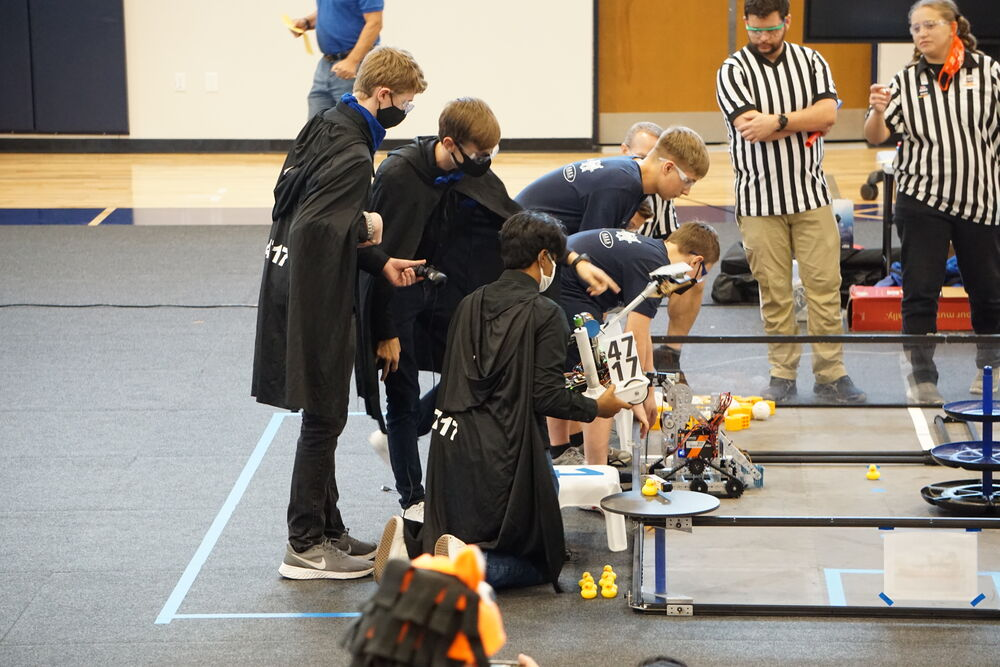
\includegraphics[width=0.95\textwidth]{Meetings/November/11-14-21/11-16-21_Team_Figure1 - Nathan Forrer.JPG}
  \caption{Meet 1}
  \label{fig:111421_1}
\end{minipage}%
\hfill%
\begin{minipage}[b]{.48\textwidth}
  \centering
  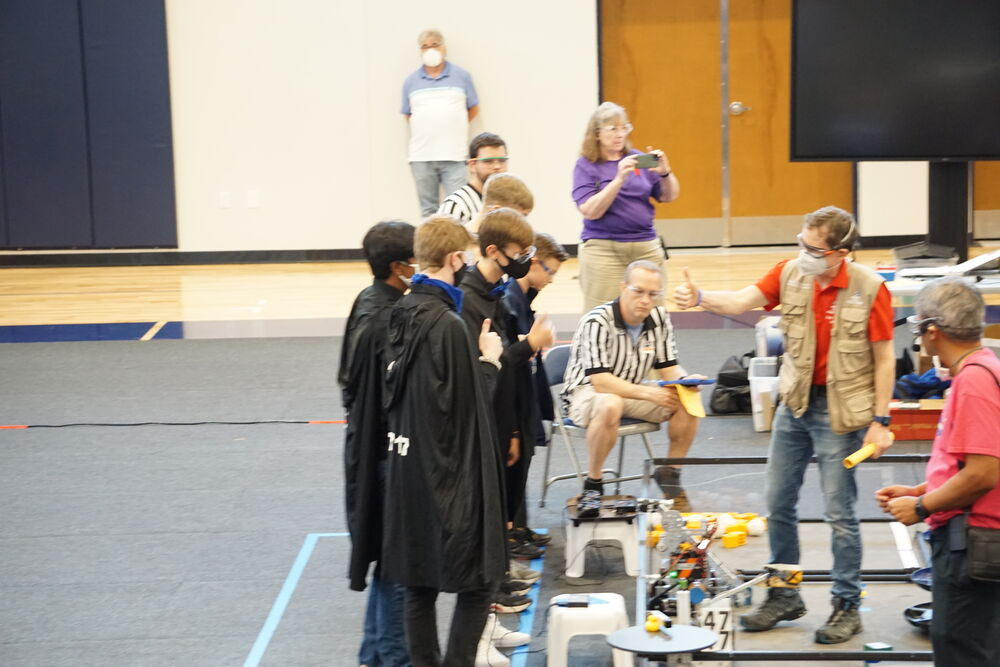
\includegraphics[width=0.95\textwidth]{Meetings/November/11-14-21/11-16-21_Team_Figure2 - Nathan Forrer.JPG}
  \caption{Meet 1}
  \label{fig:111421_2}
\end{minipage}
\end{figure}

\begin{figure}[ht]
\centering
\begin{minipage}[b]{.48\textwidth}
  \centering
  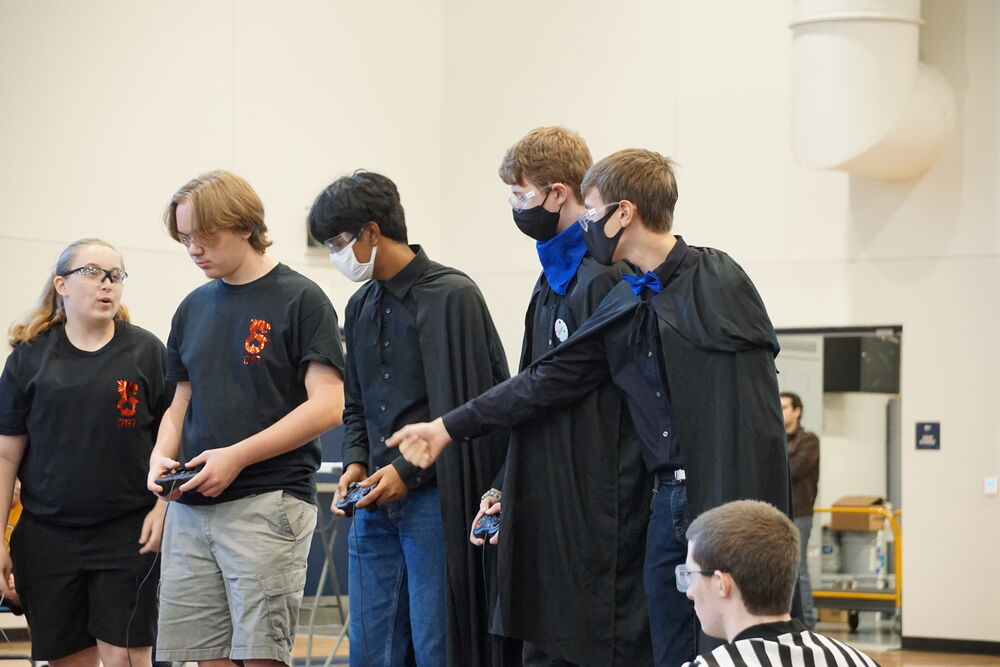
\includegraphics[width=0.95\textwidth]{Meetings/November/11-14-21/11-16-21_Team_Figure3 - Nathan Forrer.JPG}
  \caption{Meet 1}
  \label{fig:111421_3}
\end{minipage}%
\hfill%
\begin{minipage}[b]{.48\textwidth}
  \centering
  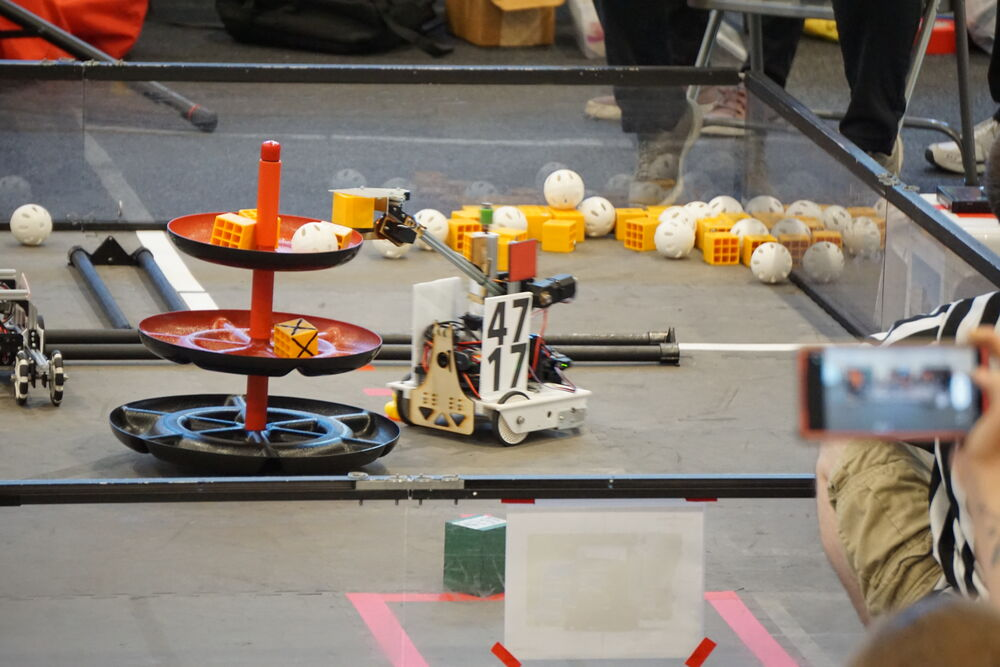
\includegraphics[width=0.95\textwidth]{Meetings/November/11-14-21/11-16-21_Team_Figure4 - Nathan Forrer.JPG}
  \caption{Meet 1}
  \label{fig:111421_4}
\end{minipage}
\end{figure}


\begin{figure}[htp]
\centering
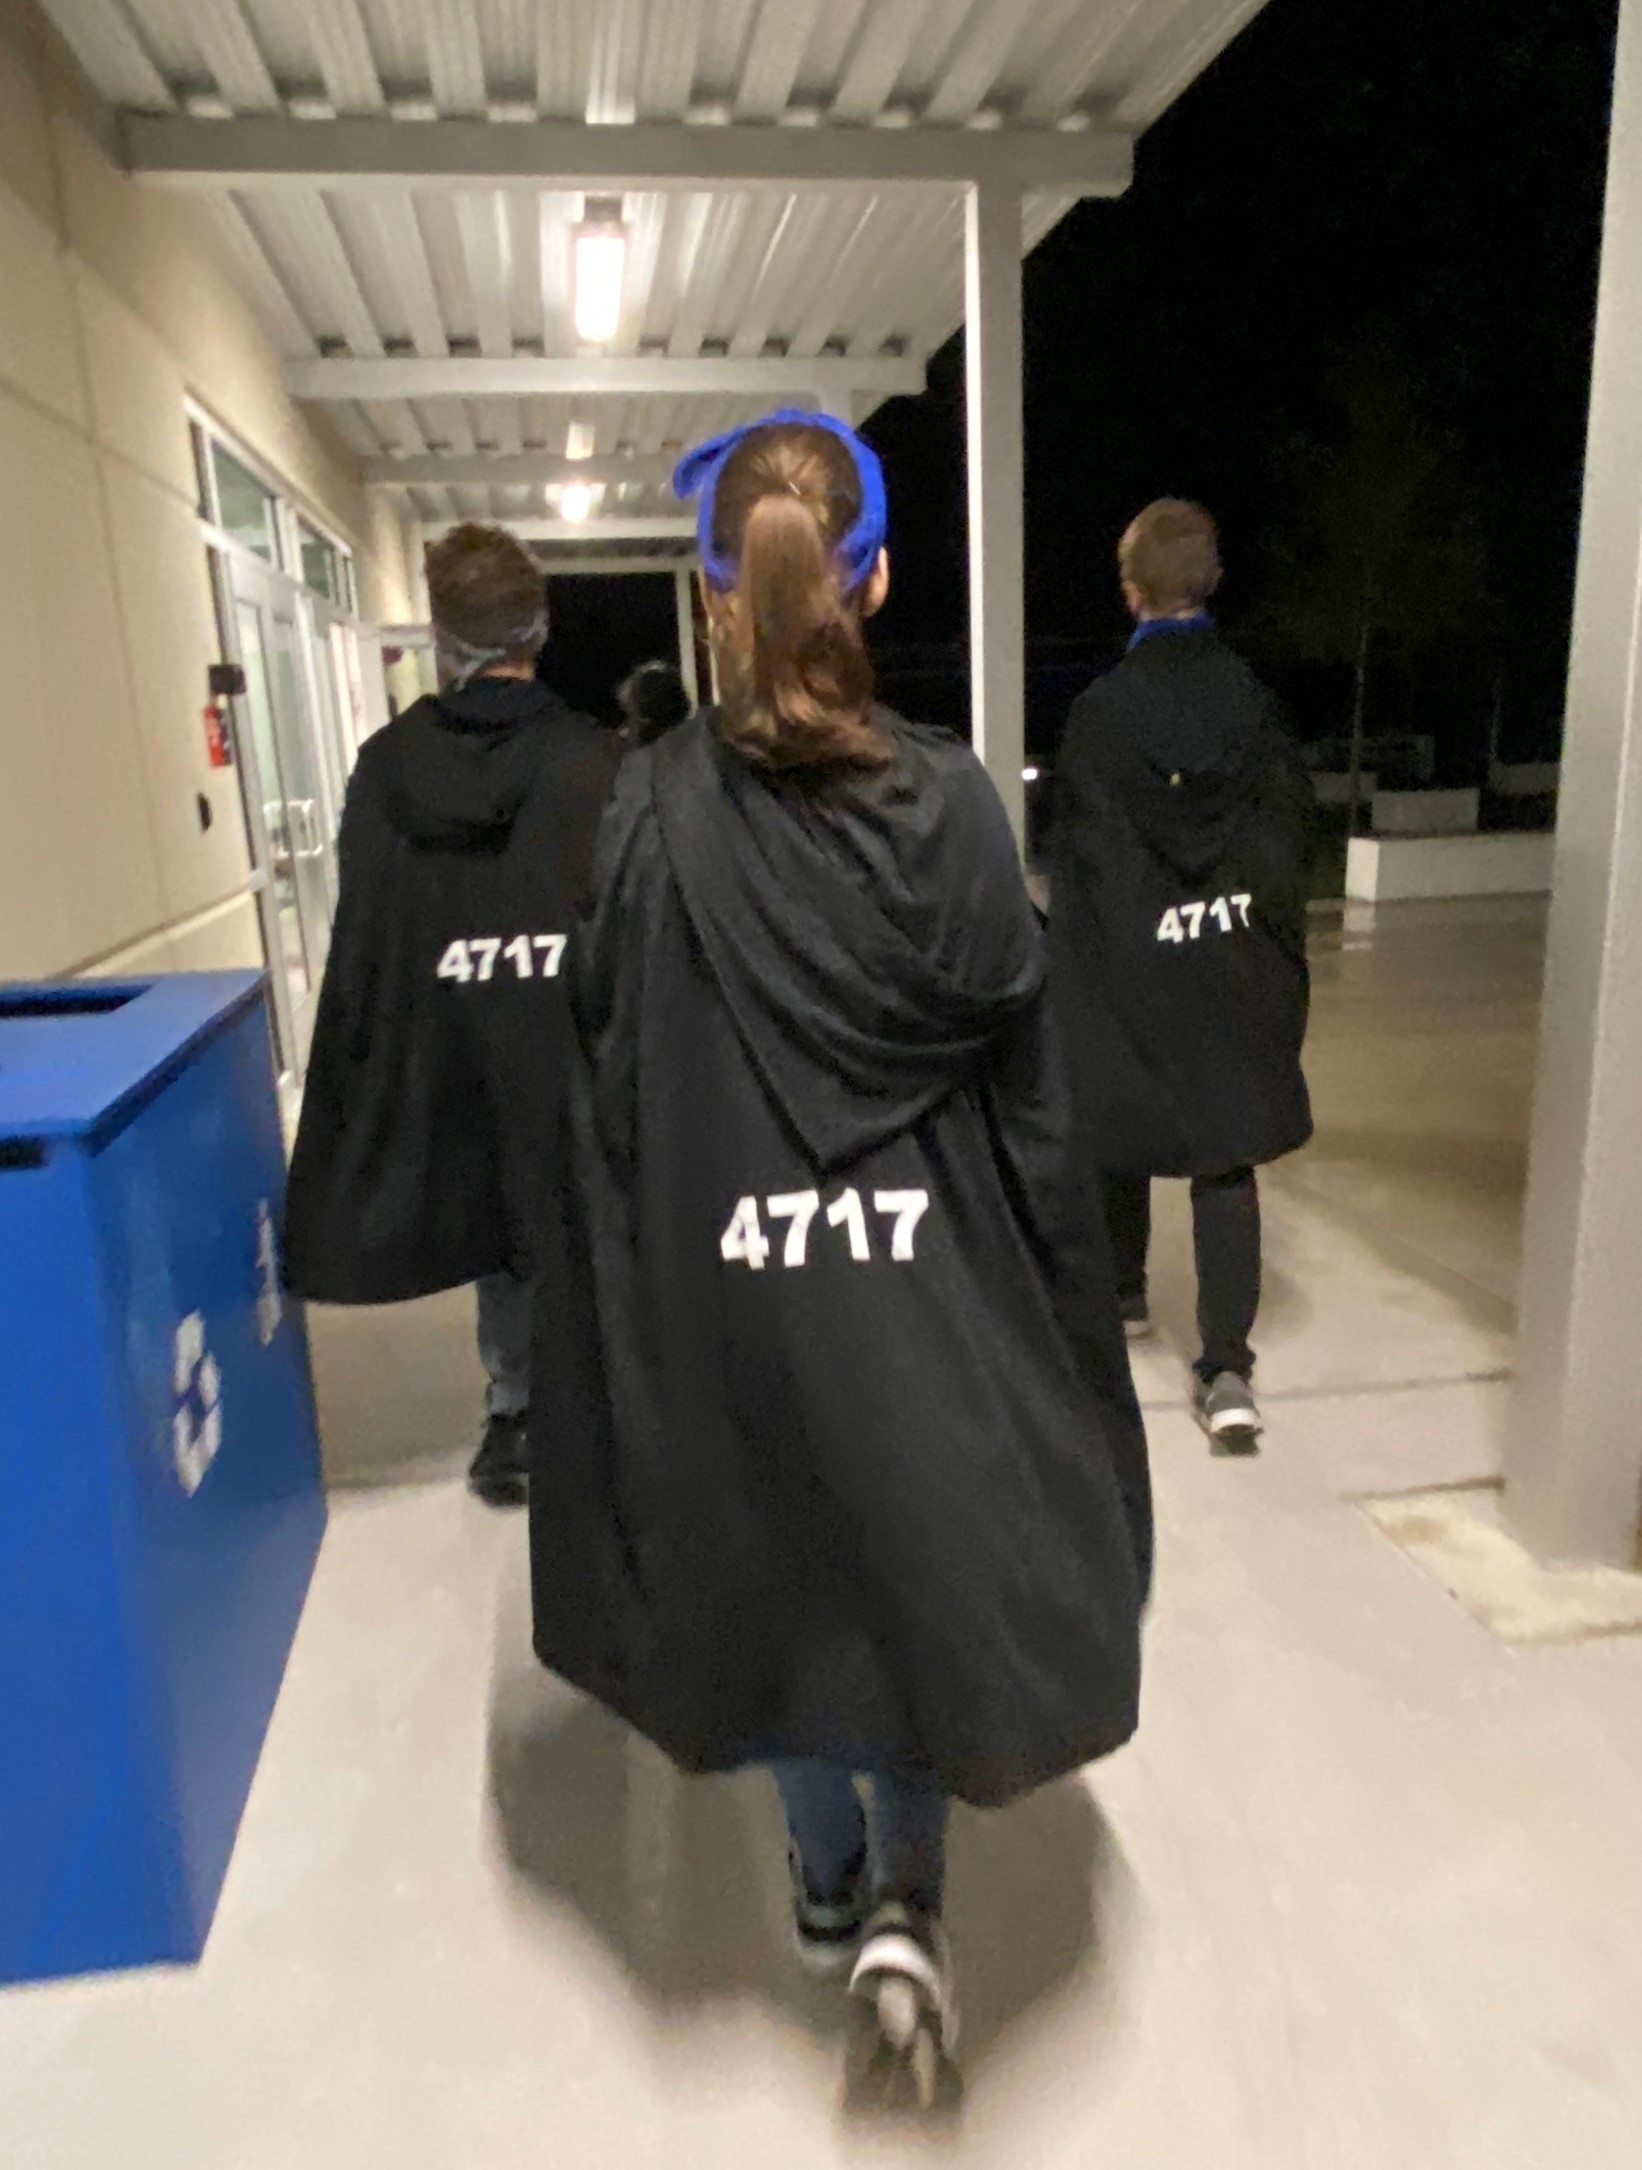
\includegraphics[width=0.95\textwidth, angle=0]{Meetings/November/11-14-21/11-16-21_Team_Figure5 - Nathan Forrer.JPG}
\caption{Meet 1}
\label{fig:111421_5}
\end{figure}



\whatsnext{
\begin{itemize}
    \item Address design issues found during meet 1
    \item Spend time doing driver practice before meet 2
\end{itemize} 
}

